\documentclass[11pt,compress,t,notes=noshow, aspectratio=169, xcolor=table]{beamer}

\usepackage{../../style/lmu-lecture}
% Defines macros and environments
% This file is included in slides and exercises

% Rarely used fontstyle for R packages, used only in 
% - forests/slides-forests-benchmark.tex
% - exercises/single-exercises/methods_l_1.Rnw
% - slides/cart/attic/slides_extra_trees.Rnw
\newcommand{\pkg}[1]{{\fontseries{b}\selectfont #1}}

% Spacing helpers, used often (mostly in exercises for \dlz)
\newcommand{\lz}{\vspace{0.5cm}} % vertical space (used often in slides)
\newcommand{\dlz}{\vspace{1cm}}  % double vertical space (used often in exercises, never in slides)
\newcommand{\oneliner}[1] % Oneliner for important statements, used e.g. in iml, algods
{\begin{block}{}\begin{center}\begin{Large}#1\end{Large}\end{center}\end{block}}

% Don't know if this is used or needed, remove?
% textcolor that works in mathmode
% https://tex.stackexchange.com/a/261480
% Used e.g. in forests/slides-forests-bagging.tex
% [...] \textcolor{blue}{\tfrac{1}{M}\sum^M_{m} [...]
% \makeatletter
% \renewcommand*{\@textcolor}[3]{%
%   \protect\leavevmode
%   \begingroup
%     \color#1{#2}#3%
%   \endgroup
% }
% \makeatother


\title{Interpretable Machine Learning}
% \author{LMU}
%\institute{\href{https://compstat-lmu.github.io/lecture_iml/}{compstat-lmu.github.io/lecture\_iml}}
\date{}

\begin{document}

\newcommand{\titlefigure}{figure/performance_vs_interpretability}
\newcommand{\learninggoals}{
\item Why interpretability?
\item Developments until now?
\item Use cases for interpretability}

\lecturechapter{Introduction, Motivation, and History}
\lecture{Interpretable Machine Learning}

\begin{frame}{Why Interpretability?}
% 		\begin{itemize}
% 			\item Machine learning (ML) has a huge potential to aid the decision-making process in various applications.
% 			\pause
% 			\smallskip
% 			\item ML models often are intransparent black boxes, e.g., XGBoost, RBF SVM, or NNs.
% 			\begin{itemize}
% 				\item[$\rightarrow$] too complex to be understood by humans.
% 			\end{itemize}
% 			\smallskip
% 			\item A lack in explanations diminishes trust in the model and creates barriers for adoption, especially in areas with critical decision-making consequences, e.g., medicine.
% 			\smallskip
% 			\item Such disciplines often rely on traditional models,\\ e.g., linear models, with less predictive performance.
% 			\smallskip
% 			\item Interpretable machine learning (IML) aims to bridge the gap between interpretability and predictive performance.
% 		\end{itemize}
%\bigskip
    \begin{columns}[T, totalwidth=\textwidth]
    \begin{column}{0.8\textwidth}
		\begin{itemize}
			\item ML: huge potential to aid decision-making process due to its predictive performance
			%\pause
			%\smallskip
			\item ML models are black boxes, e.g., XGBoost, RBF SVM or DNNs \\ 
            $\leadsto$ too complex to be understood by humans
			\item Some applications are "learn to understand"
			%\pause
			%\smallskip
			\item<2-> When deploying ML models, lack of explanations 
			\begin{enumerate}
				\item hurts trust
				\item creates barriers
			\end{enumerate}
			%\only<4->{\item[$\leadsto$] Hard to adapt in critical areas when decisions affect human life}
			\item<2->[\,$\leadsto$] Many disciplines with required trust rely on traditional models,\\ e.g., linear models, with less predictive performance   
		\end{itemize}
    \centering\includegraphics<2->[width=0.7\textwidth]{figure/performance_vs_interpretability.pdf}
    % Quelle: https://docs.google.com/presentation/d/1Ah4fTi11bJITOIomtm71NPp0Wko5D5wzZYcL-Htm7qk/edit?usp=sharing
    %\centering \citebutton{Scott Fortmann-Roe (2012)}{http://scott.fortmann-roe.com/docs/BiasVariance.html}
	\end{column}
	\begin{column}{0.2\textwidth}  %%<--- here
        \centering
        \includegraphics[width=0.9\textwidth]{figure/nn_model.png}
        \includegraphics[width=0.9\textwidth]{figure/nn_landscape.png}
        %\centering \citebutton{Liu 2021}{https://davideliu.com/2021/12/12/visualizing-loss-landscape-of-gail/}
    \end{column}
    \end{columns}
    % \bigskip
    % \begin{columns}[T, totalwidth=\textwidth]
    %     \begin{column}{0.5\textwidth}
    %     \begin{itemize}
    %         \only<5>{\item[$\leadsto$] Harder to adapt for critical areas with decisions affecting human life}
    %         \item<5>[\,$\leadsto$] Many disciplines with required trust rely on traditional models,\\ e.g., linear models, with less predictive performance
    %     \end{itemize}
    %     \end{column}
	   % \begin{column}{0.5\textwidth} 
	   %     \only<5>{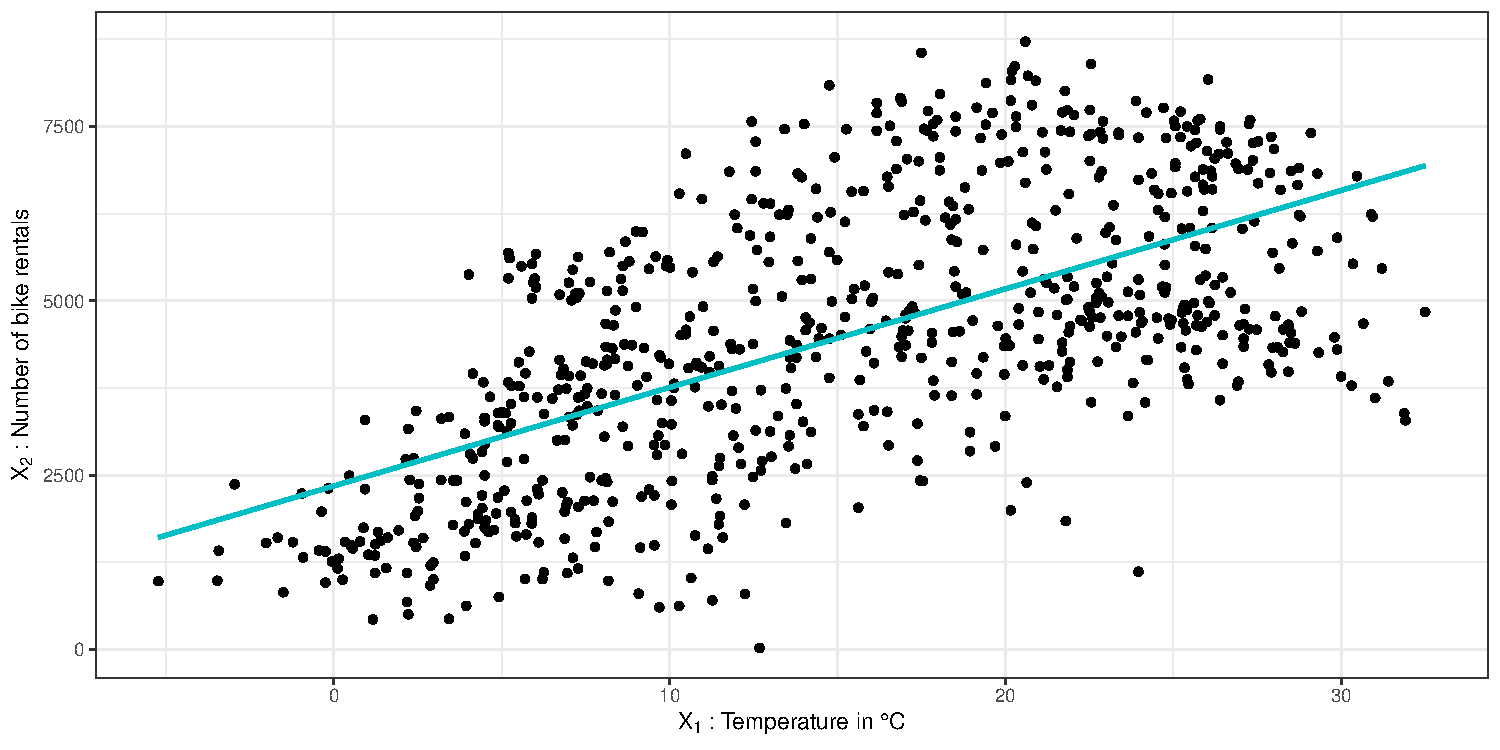
\includegraphics[width=\textwidth]{figure/intro_lm_bike.pdf}}
	   % \end{column}
    %     \end{columns}
\end{frame}
	
	
\begin{frame}{Interpretability in High-stakes Decisions}

Examples of critical areas where decisions based on ML models can affect human life 
    % \begin{itemize}
    %     \item Credit scoring and insurance applications
    %     \citebutton{Society of Actuaries}{https://www.soa.org/resources/research-reports/2021/interpretable-machine-learning}
    % \end{itemize}
    \begin{columns}[T, totalwidth=\textwidth]
    \begin{column}{0.55\textwidth}
		\begin{itemize}
		\item Credit scoring and insurance applications
        \citebutton{Society of Actuaries}{https://www.soa.org/resources/research-reports/2021/interpretable-machine-learning}
        \begin{itemize}
            \item Reasons for not granting a loan
            \item Fraud detection in insurance claims
        \end{itemize}
    \end{itemize}
    \end{column}
	\begin{column}{0.45\textwidth}
        \centering
        \includegraphics<1->[page=1, width=.95\textwidth, trim = 0 250 0 0, clip]{figure/counterfactual.pdf}
	\end{column}
    \end{columns}
    \bigskip
    \begin{columns}[T, totalwidth=\textwidth]
    \begin{column}{0.55\textwidth}
		\begin{itemize}
		\item<2-> Medical applications
        \begin{itemize}
            \item Identification of diseases
            %\item Chance of recovering
            \item Recommendations of treatments
        \end{itemize}
        \item<2-> \ldots
    \end{itemize}
    \end{column}
	\begin{column}{0.45\textwidth}
        \centering
        \only<2->{\includegraphics[width=\textwidth]{figure/medicine.png}
	    \citebutton{Miliard (2020)}{https://www.healthcareitnews.com/news/new-ai-diagnostic-tool-knows-when-defer-human-mit-researchers-say}}
	\end{column}
    \end{columns}
\end{frame}


\begin{frame}{Need for interpretability}

    Need for interpretability becoming increasingly important from a legal perspective
    
    \begin{itemize}
    \item General Data Protection Regulation (GDPR) requires for some applications that models have to be explainable \citebutton{Goodman \& Flaxman (2017)}{https://doi.org/10.1609/aimag.v38i3.2741}\\
    $\leadsto$ \textit{EU Regulations on Algorithmic Decision-Making and a ``Right to Explanation''} 
    
    \item \textit{Ethics guidelines for trustworthy AI}
    \citebutton{European Commission (2019)}{https://doi.org/10.2759/346720}

    \end{itemize}
    \medskip
    
    \centering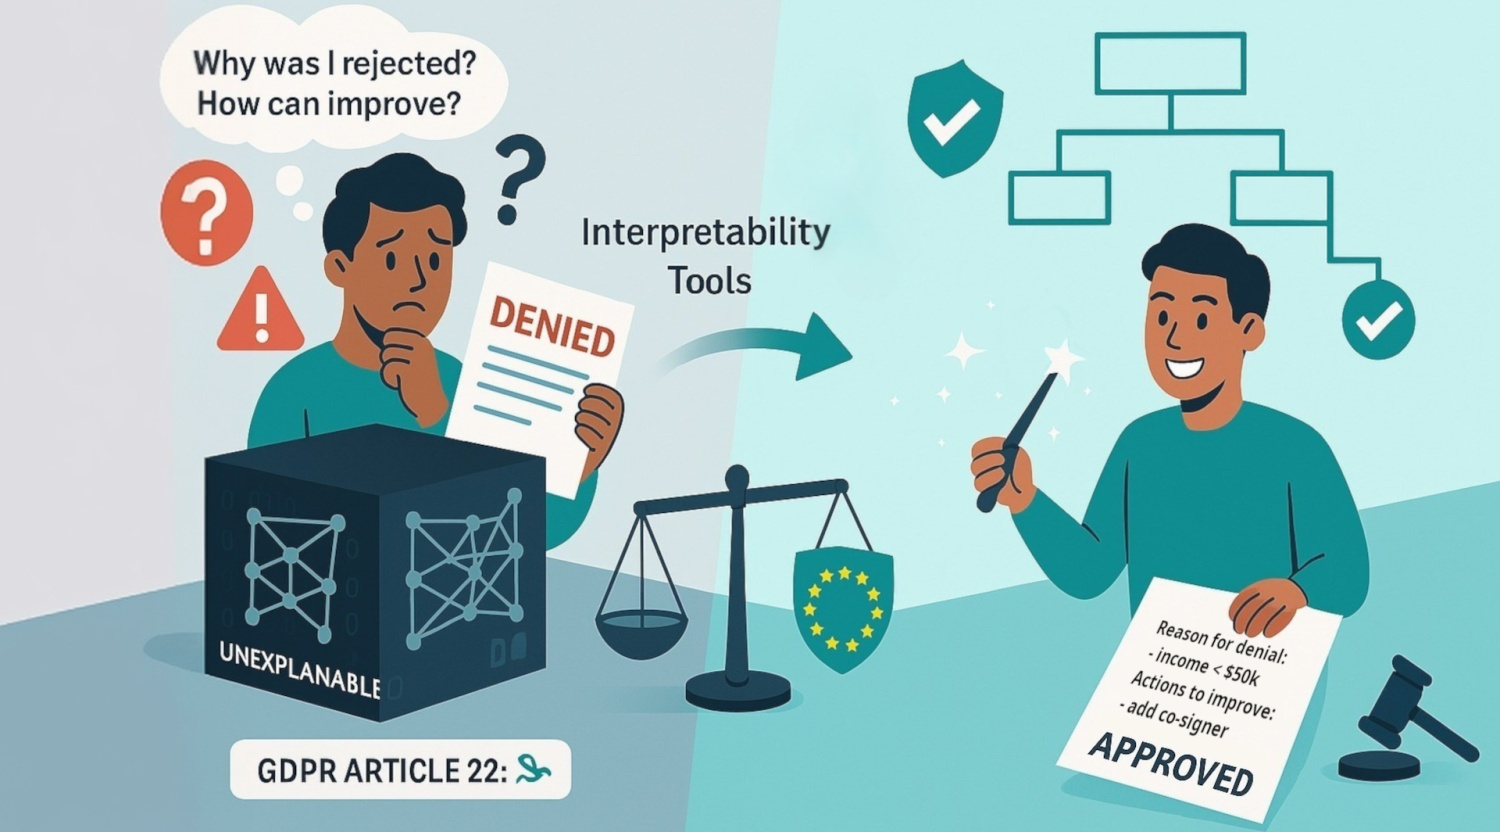
\includegraphics[width=0.85\textwidth]{figure/rightstoexplain.jpg}
    % source https://www.propublica.org/article/how-we-analyzed-the-compas-recidivism-algorithm
\end{frame}



% \begin{frame}{Performance vs. Interpretability}
%     \centering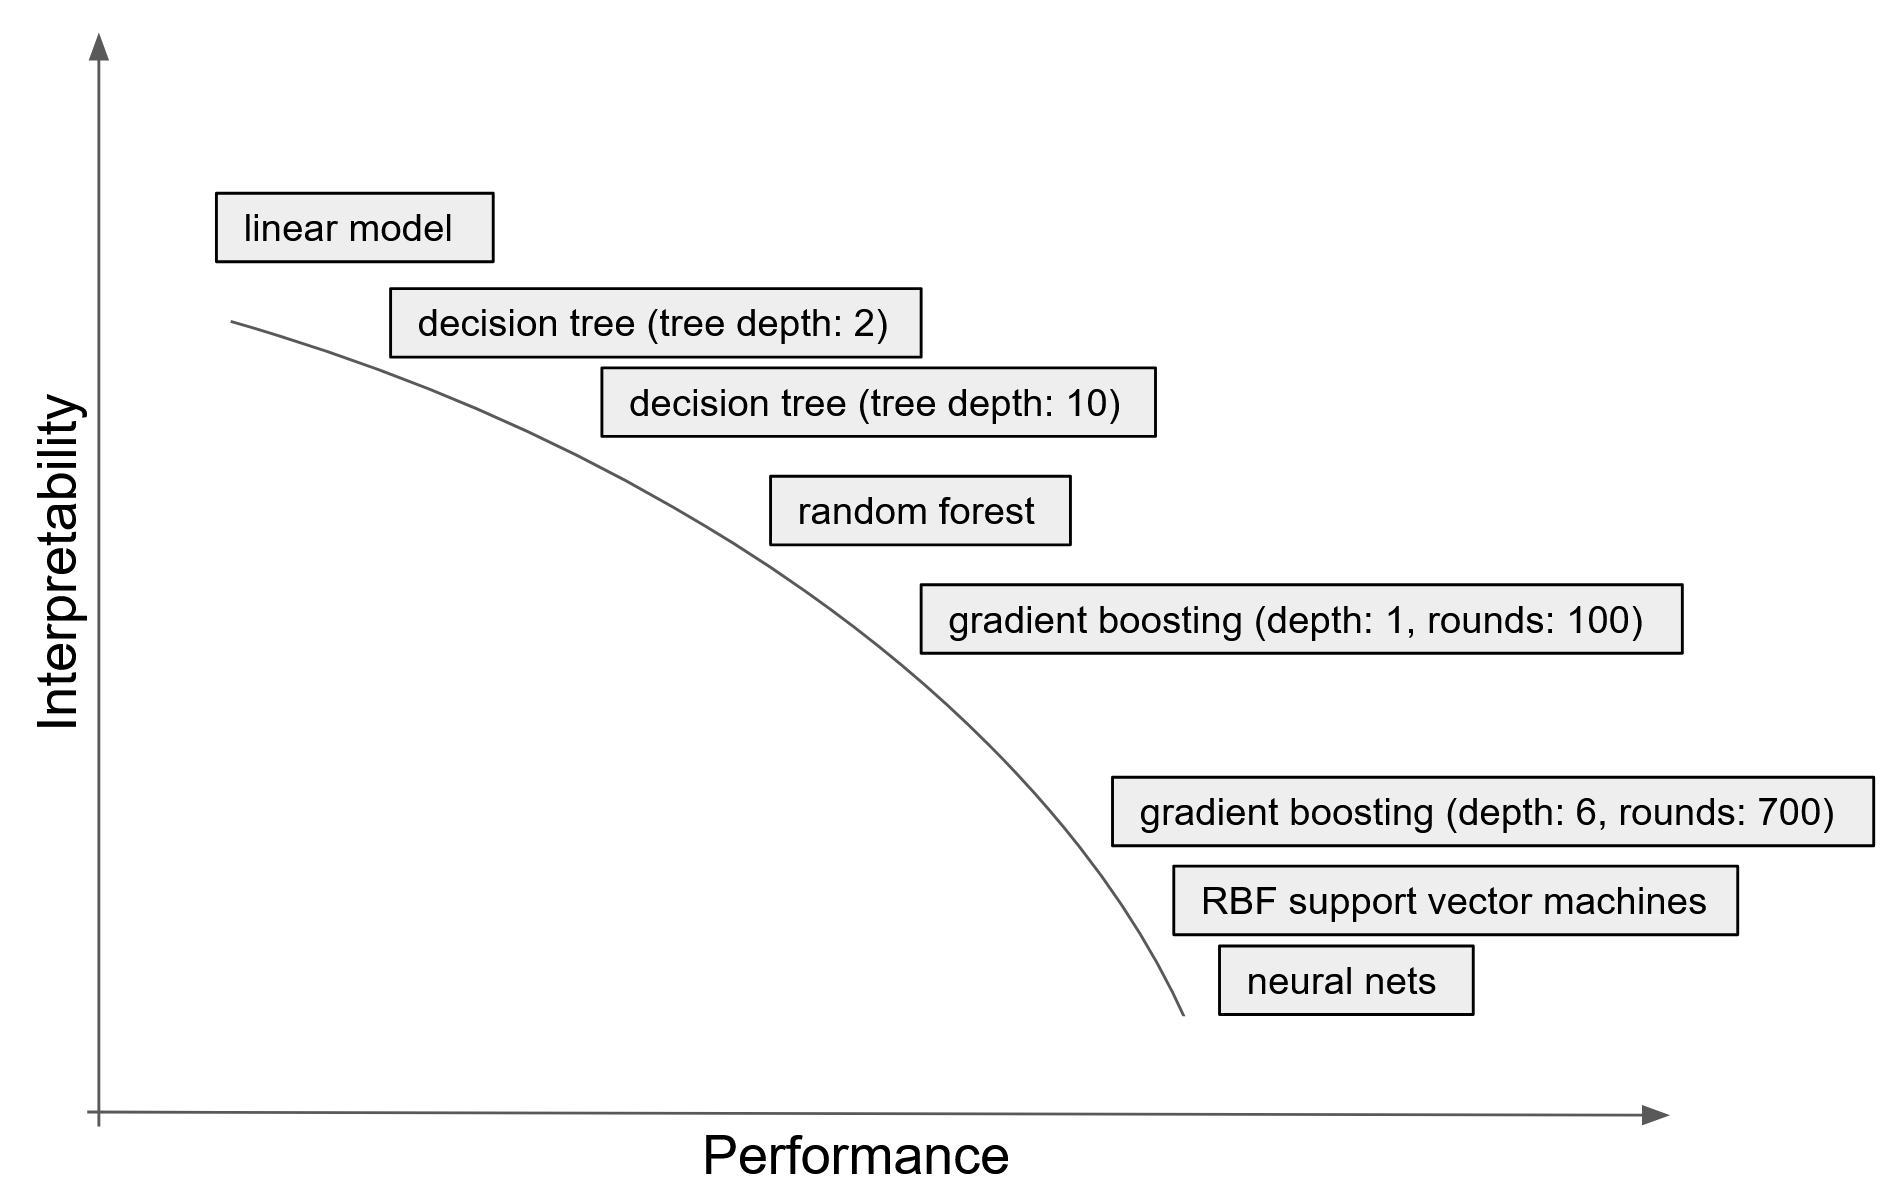
\includegraphics[width=0.7\textwidth]{figure/performance_vs_interpretability.png}
%     % Quelle: https://docs.google.com/presentation/d/12ZPrTjBKEUT-7drdyUJCQGK0oHVDtYIVd2_6byE62f0/edit?usp=sharing
%     %\centering \citebutton{Scott Fortmann-Roe (2012)}{http://scott.fortmann-roe.com/docs/BiasVariance.html}
% \end{frame}


	%-----------------------------------------------------------------------------------------------------------------------------

\begin{frame}{Brief History of Interpretability}
	\begin{columns}[T, totalwidth=\textwidth]
	\begin{column}{0.75\textwidth}
	    \begin{itemize}
			\item 18th and 19th century: \\Linear regression models (Gauss, Legendre, Quetelet)
			\medskip
			\item 1940s:\\ Emergence of sensitivity analysis (SA)
			\medskip
			\item Middle of 20th century:\\ Rule-based ML, incl. decision rules and decision trees
			\medskip
			\item 2001:\\ Built-in feature importance measure of random forests
			\medskip
			\item >2010: \\Explainable AI (XAI) for deep learning
			\medskip
			\item >2015: \\IML as an independent field of research
		\end{itemize}
	\end{column}
	\begin{column}{0.25\textwidth}
	    \includegraphics[width=0.8\textwidth]{figure/Carl_Friedrich_Gauss_1828.jpg}
        \centering \citebutton{Carl Friedrich Gauss}{https://commons.wikimedia.org/w/index.php?curid=2404149}
        \centering \citebutton{Wikipedia}{https://en.wikipedia.org/wiki/Carl_Friedrich_Gauss}
        \bigskip\\
        \includegraphics[width=0.9\textwidth]{figure/Random_Forest.png}
        % https://docs.google.com/presentation/d/15HjwMHdTtZ9N0cniUPsiztRSRg1UDY3Y5M8tXsaqt2I/edit?usp=sharing
	\end{column}
	\end{columns}
\end{frame}

\endlecture
\end{document}
